\documentclass[titlepage]{report}
\usepackage[ngerman]{babel}
\usepackage[backend=biber,style=numeric]{biblatex}
\addbibresource{literature.bib}
\usepackage{caption}
\usepackage{subcaption}
\usepackage{graphicx}
\usepackage[utf8]{inputenc}
\usepackage[T1]{fontenc}
\usepackage{url}
\usepackage{hyphenat}
\usepackage{glossaries}
\usepackage{array}
\usepackage{calc}
\usepackage{booktabs}
\usepackage{hyperref}
\makeglossaries{}
\newglossaryentry{dns}
{%
    name={DNS},
    description={},
    first={Domain Name System (DNS)},
    long={Domain Name System}
}

\newglossaryentry{http}
{%
    name={HTTP},
    description={},
    first={Hypertext Transport Protocol (HTTP)},
    long={Hypertext Transport Protocol}

}
\newglossaryentry{https}
{%
    name={HTTPS},
    description={},
    first={Hypertext Transport Protocol Secure (HTTPS)},
    long={Hypertext Transport Protocol Secure}

}
\newglossaryentry{cifs}
{%
    name={CIFS},
    description={},
    first={Common Internet File System (CIFS)},
    long={Common Internet File System}

}
\newglossaryentry{voip}
{%
    name={VoIP},
    description={},
    first={Voice Over Internet Protocol (VoIP)},
    long={Voice Over Internet Protocol}

}
\newglossaryentry{tuc}
{%
    name={TU Clausthal},
    description={},
    first={Technische Universität Clausthal},
}
\newglossaryentry{efzn}
{%
    name={EFZN},
    description={},
    first={Energie-Forschungszentrum Niedersachsen (EFZN)},
    long={Energie-Forschungszentrum Niedersachsen}
}
\newglossaryentry{rfc}
{%
    name={RFC},
    description={},
    first={Request For Comments (RFC)},
    long={Request For Comments}
}

\title{Evaluierung eines Messpunkte-Clusters für Netzwerktests auf dem
Campus der TU Clausthal}
\author{Christian, Rebischke\\
\gls{tuc}\\
Rechenzentrum\\
Email: Christian.Rebischke@tu-clausthal.de}
\begin{document}
\maketitle
\chapter*{Danksagung}
Ich bedanke mich bei dem Rechenzentrum der \gls{tuc}, insbesondere bei
Dipl.\hyp{}Math. Christian Strauf. Das Thema dieser Bachelorarbeit
beruht auf seiner Idee und war mein Ansporn mich mit diesem Thema näher
auseinanderzusetzen. Desweiteren danke ich Herrn Prof. Dr.\hyp{}Ing. Dr.
rer. nat. habil. Harald Richter für die Unterstützung aus akademischer
Seite. Besonderen Dank bekommt von mir auch die Opensource Gemeinschaft.
Ohne die harte Arbeit der Opensource Gemeinschaft würden die grundlegenden
Werkzeuge die ich zur Vollendung dieser Bachelor-Arbeit benutzt habe
nicht existieren. Darunter das Softwarepaket \LaTeX, die Zeichensoftware
\emph{Draw IO} (\url{https://www.draw.io/}) und viele weitere spannende
freiverfügbare Projekte.
\tableofcontents
\chapter*{Vorwort}
\addcontentsline{toc}{chapter}{Vorwort}
Es gibt nun seit mehr als 20 Jahren das Internet und keine Technologie
ist wohl über so kurze Zeit so alltäglich geworden. Das Internet hat es
geschafft Einzug zu erhalten in Arbeit, Privatleben und auch Forschung
und Lehre. Nahezu in allen wissenschaftlichen Diszplinen spielt das
Internet und die damit verknüpfte Informationstechnologie eine Rolle.
Sei es die Industrie 4.0 mit ihren Cyber-physischen Systemen, dem
schnellen Abgleich von DNA-Informationen über das Netz in der
angewandten Biologie, dem Sammeln von Krankheitsdaten in der Medizin
oder das Verarbeiten von Datenmengen gigantischen Ausmaßes im
Finanzsektor. All diese Beispiele sind nur möglich durch immer größere
Technologiesprünge in der Informatik und dem immer weiteren Ausbau des
Internets. Da ist es nicht verwunderlich, dass der UN-Menschenrechtsrat das
Internet zu einem Menschenrecht\cite{UNHRC} erklärt hat und umso weniger
verwunderlich ist es, dass die Vernetzung von Computersystemen auch auf
dem Campus der \gls{tuc} eine Rolle spielt,
nicht nur für Forschung und Lehre, sondern natürlich auch für den
täglichen Betrieb. Eine Schlüsselposition nimmt dabei das Rechenzentrum
der \gls{tuc} ein. Das Rechenzentrum bildet die
Basis für die Vernetzung der einzelnen Fakultäten untereinander, die
Vernetzung zwischen Fakultäten und Firmen aus der freien Wirtschaft,
sowie auch die Vernetzung zwischen der \gls{tuc}
und anderen Universitäten weltweit. Dementsprechend wichtig ist ein
stabiles Netz für den täglichen Betrieb. In dieser Bachelorarbeit widme
ich mich deshalb der technischen Umsetzung eines verteilten
Monitoring-Systems zur Überwachung der Netzwerkqualität zwischen
einzelnen Endpunkten und Kernsystemen die für einen problemlosen
Netzbetrieb nötig sind. Das Rechenzentrum der \gls{tuc} dient bei dieser
Bachelorarbeit als Auftraggeber.
\chapter*{Problemstellung}
\addcontentsline{toc}{chapter}{Problemstellung}
Das Netz der \gls{tuc} erstreckt sich über mehrere
Standorte. Teilweise liegen diese Standorte nicht in Clausthal
selbst, wie beispielsweise das \gls{efzn} in Goslar. Dementsprechend
schwierig gestaltet sich die Wartung und der Betrieb
des Netzes. So kann auf Netzeinbrüche etwa nur reaktiv
nach Meldung des Problems reagiert werden. Es existiert
zwar ein Monitoring-System, welches die Verfügbarkeit von
einzelnen Diensten überprüft, jedoch erfolgt diese Messung
nur von einem Punkt aus und gibt nur binäre Statuswerte
zurück (Dienst läuft oder Dienst läuft nicht). Dementsprechend
fehlen Informationen um die Verfügbarkeit von Diensten und
deren vollständige Funktion von mehreren Messpunkten aus
zu garantieren. Beispielsweise ist es möglich, dass ein Dienst
zwar vom zentralen Monitoring-Server aus erreichbar ist, aber
aus einem einzelnen Institut der Zugriff auf den Dienst nur
eingeschränkt oder sogar gar nicht möglich ist. Das Rechenzentrum der
\gls{tuc} bietet mehrere Kerndienste an. Dazu
gehören:
\begin{itemize}
    \item \gls{dns}
    \item Diverse Webdienste basierend auf:
    \begin{itemize}
        \item \gls{http}
        \item \gls{https}
    \end{itemize}
    \item \gls{cifs}
    \item \gls{voip}
\end{itemize}
Besonders Dienste wie \gls{dns} sind auf schnelle
Verbindungen angewiesen. Eine zu hohe Latenz zwischen einem Client und
dem Dienst führt unweigerlich zu für den Nutzer sichtbaren Konsequenzen
(zum Beispiel verzögerte Seitenaufrufe beim Web-Browsing). Noch mehr ins
Gewicht fallen Latenzen bei \gls{voip}, dort sind Latenzen
oder ein Jitter (die Varianz der Laufzeit der Datenpakete\cite{JITTERWIKI})
leicht auszumachen. Nämlich an abgehakten Telefonaten oder Rauschen in
der Leitung. Was also fehlt ist ein Netz aus verteilten Messpunkten,
dass es ermöglicht die Erreichbarkeit einzelner Dienste periodisch und
über einen längeren Zeitraum zu beobachten. Dies hätte zwei Vorteile.
Zum einen lässt sich so der Zustand des Campus-Netzwerks besser
erfassen, da Tests nicht nur von einem zentralen Monitoring-System aus
gestartet werden. Zum anderen können die gewonnenen Daten weiter
verwertet, grafisch aufbereitet und zum Beispiel für die Erstellung von
Langzeitstatistiken über die Gesundheit des Netzwerks genutzt werden.
Weiterhin könnten im Fall eines Ausfalls natürlich die zuständigen
Netzadministratoren benachrichtigt werden, im Idealfall durch gewohnte
Kommunikationswege wie Email. Mit dem Wandel von einem zentralen zu
einem dezentralen Monitoring-System entsteht allerdings auch mehr
Arbeitsaufwand. Denn auch diese Systeme müssen gewartet werden. Im
nachfolgenden Kapitel werden aus dieser Problemstellung die nötigen
Anforderungen abgeleitet und ein erster Lösungsansatz für das Problem
erstellt.
\chapter*{Technische Grundlagen}
\addcontentsline{toc}{chapter}{Technische Grundlagen}
In diesem Kapitel werden die für die Lösung des Problems nötigen
technischen Grundlagen erläutert. Darunter fallen einige wichtige
Protokolle.
\section*{\glsfirst{dns}}
\addcontentsline{toc}{section}{\glsfirst{dns}}
Aus Erfahrungen mit dem Internetvorgänger \gls{arpanet} wurde
abgeleitet, dass ein manuelles Eingeben von \gls{ip}\hyp{}adressen mit
steigender Anzahl von Knoten im Netzwerk immer unübersichtlicher wurde.
Hinzukommend sind \gls{ip}\hyp{}Adressen für den Menschen schwer zu
merken. Mit dieser Problemstellung als Grundlage arbeitete der Ingenieur
Peter Mockapetris an einem ersten Lösungsansatz: \glsfirst{dns}.
Bei \gls{dns} handelt es sich um einen mehr als 20 Jahre alten
Verzeichnisdienst, welcher über das gleichnamige Protokoll, für Menschen
merkbare Internetadressen auf \gls{ip}\hyp{}Adressen abbildet.
\gls{dns} wurde erstmalig im Jahr 1983 in den beiden \glspl{rfc}
\gls{rfc} 882\cite{RFC0882} und \gls{rfc} 883\cite{RFC0883} beschrieben.
Damals befanden sich die \gls{dns}\hyp{}Einträge, die Abbildungen von
lesbarer Adresse auf \gls{ip}\hyp{}Adresse, noch verteilt auf
allen Servern des frühen Internets und wurden von der \gls{nic} verwaltet
und mit dem Dateiübertragungsprotokoll \gls{ftp}
synchronisiert\cite{RFC1034}. In der damaligen Zeit stellte sich dies
als ein Flaschenhals für das Internet heraus, da die Anzahl der Server
im Netzwerk exponentiell zunahm. Deshalb wurden nur vier Jahre später
Überarbeitungen von \gls{dns} veröffentlicht. Diese Überarbeitungen
wurden in den \glspl{rfc} \gls{rfc} 1034 und \gls{rfc} 1035 erläutert
und bilden die Grundlage für \gls{dns} wie es heute bekannt ist und auch
eingesetzt wird. Der heutige Ansatz verläuft dezentraler als es damals
der Fall gewesen ist. Anstatt die \gls{dns}\hyp{}Einträge auf allen
Knoten des Internets zu verteilen und zentral von der \gls{nic} aus zu
steuern, existieren heute mehrere hierarchische Verwaltungsebenen. Dazu
wird der \gls{fqdn} hierarchisch gegliedert. Ein Beispiel für einen
\gls{fqdn} ist beispielsweise \emph{akira.rz.tu-clausthal.de}. Die
\autoref{fig:1} veranschaulicht, die Gliederung dieses \gls{fqdn} in die
einzelnen Bestandteile.
\newpage
\begin{figure}[h]
    \centering
    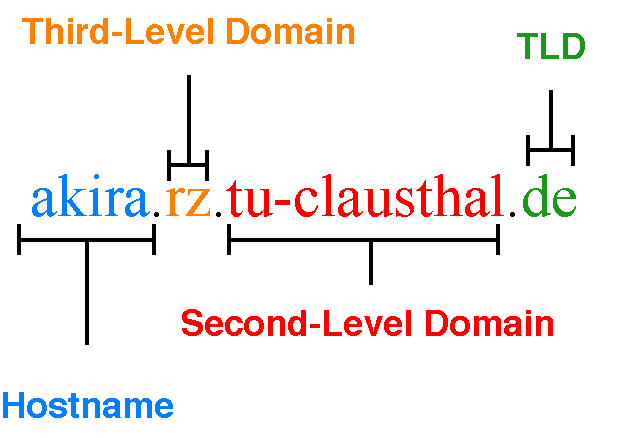
\includegraphics[width=0.5\textwidth]{figures/dnsname.pdf}
    \caption{Bestandteile eines \gls{fqdn} mit optionalem Hostname und Third-Level
    Domain}\label{fig:1}
\end{figure}
Eine Angabe des Hostname oder einer Third-Level
Domain ist optional. Es können auch weitere Domains hinzugefügt werden.
So ist auch eine Sixth-Level Domain möglich. Die Maximale Anzahl der
Subdomains ist in keinem der \gls{dns} \glspl{rfc} spezifiziert. Deshalb
ist die maximale Anzahl abhängig vom \gls{dns}\hyp{}Server der die
Domains ausliefert. Nach \gls{rfc} 1035 ist die maximale Länge eines
\gls{fqdn} aber auf 255 Bytes begrenzt\cite[siehe Section
2.3.4]{RFC1035}, was die maximale Anzahl von Subdomains zumindest stark
einschränkt. Der Begriff Subdomain umfasst alle Domains unter der
\gls{tld}. \glspl{fqdn} sind nicht nur hierarchisch strukturiert, sondern
unterliegen zusätzlich einer Baumstruktur. Dessen Wurzel ist die
\emph{Root Domain}, meistens symbolisiert durch einen einfachen Punkt.
Eine Ebene direkt darunter sind die \glspl{tld} diese
werden in der Regel von den \glspl{nic} einzelner Länder verwaltet. Von
Ländern verwaltete \glspl{tld} haben meist Länderabkürzungen wie
\emph{de} (Deutschland), \emph{jp} (Japan) oder \emph{cn} (Volksrepublik
China). Es existieren aber auch militärische oder akademische
\glspl{tld} wie \emph{edu} und \emph{mil}. In Deutschland ist die DENIC eG
verantwortlich für Domains mit \emph{de}\hyp{}Endung.
In den letzten 5 Jahren kamen auch noch neue \glspl{tld} hinzu, welche
nicht an Länder geknüpft sind. Darunter fallen Markennamen wie
\emph{BMW}, \emph{Audi} oder \emph{Deutschepost} oder markenfreie Namen
wie \emph{academy}, \emph{fun} oder \emph{house}\cite{NEWTLDLIST}. Die
Vergabe der \glspl{tld} verlief direkt über die \gls{icann}. Der jeweilige
Käufer ist dann Eigentümer der jeweiligen \gls{tld}. Ein Eigentümer
einer \gls{tld} kann dann beliebig viele Subdomains erstellen für den
Eigenbedarf oder diese weiterverkaufen.
\section*{\glsfirst{http}}
\addcontentsline{toc}{section}{\glsfirst{http}}
\section*{\glsfirst{https}}
\addcontentsline{toc}{section}{\glsfirst{https}}
\section*{\glsfirst{cifs}}
\addcontentsline{toc}{section}{\glsfirst{cifs}}
\section*{\glsfirst{voip}}
\addcontentsline{toc}{section}{\glsfirst{voip}}
\chapter*{Herleitung eines Lösungsansatzes}
\addcontentsline{toc}{chapter}{Herleitung eines Lösungsansatzes}
\section*{Anforderungsanalyse}
\addcontentsline{toc}{section}{Anforderungsanalyse}
Nachfolgend werden die ermittelten funktionalen und nichtfunktionalen
Anforderungen erläutert. Funktionale Anforderungen stellen das
``eigentliche Systemverhalten und die jeweiligen Funktionen des zu
erstellenden Produkts''\cite[S. 20]{BPSE} dar, also die grundlegenden
Aufgaben der Software im Bezug auf die Problemstellung. Die
nichtfunktionalen Anforderungen dagegen sind besonders. Sie umfassen
Anforderungen wie Sicherheit, nachträgliche Erweiterbarkeit,
Testbarkeit, also Anforderungen die erst nach der Entwicklung
mess\hyp{} oder testbar werden\cite[S. 292]{SNFA}. Um die funktionalen
und nichtfunktionalen Anforderungen besser einordnen zu können, werden
folgende Schlüsselwörter zum Kennzeichnen für Anforderungen nach
\gls{rfc} 2119\cite{RFC2119} definiert:
\begin{description}
    \item[ERFORDERLICH] ist eine absolute Anforderung an die Software. Alle
        Anforderungen die mit \textbf{ERFORDERLICH} markiert sind,
        \textbf{MÜSSEN} implementiert werden.
    \item[VERBOTEN] beschreibt eine negative Anforderung. Demnach eine
        Anforderung die auf keinen Fall implementiert werden darf.
    \item[EMPFOHLEN] ist eine Anforderung die implementiert werden
        \textbf{SOLLTE} aber nicht \textbf{MUSS}. Dies ist der Fall bei
        Anforderungen die aus nachvollziehbaren Gründen nicht
        implementiert wird.
    \item[NICHT EMPFOHLEN] ist das Gegenteil von \textbf{EMPFOHLEN}. Es
        handelt sich hier um Anforderungen die vermieden werden sollten.
    \item[OPTIONAL] ist eine Anforderung die implementiert werden
        \textbf{KANN}. Diese Art von Anforderungen sind
        zusätzliches Extra und nicht nötig für die Grundfunktion der
        Software.
\end{description}
\textbf{Anmerkung}: Das \gls{rfc} 2119 ist im Original in Englisch. Ich
habe mich zur übersetzung der Schlüsselwörter auf die Übersetzung der
Schweizer Firma Adfinis SyGroup AG gestützt\cite{RFC2119DE}.
\section*{Funktionale Anforderungen}
\addcontentsline{toc}{section}{Funktionale Anforderungen}
\begin{center}
\begin{tabular}{p{0.7\textwidth-\tabcolsep}>{\raggedleft\arraybackslash}p{0.3\textwidth-\tabcolsep}}\toprule
    \textbf{FA1: Zeitmessung von \gls{dns}-Abfragen } & \textbf{Priorität: MUSS} \\\midrule
	\multicolumn{2}{p{\textwidth-\tabcolsep}}{%
    Die Software \textbf{MUSS} die Zeit messen können, die vergeht
    zwischen einer \gls{dns}-Abfrage und der Antwort von einem
    \gls{dns}-Server}\\\bottomrule
\end{tabular}
\end{center}
\begin{center}
\begin{tabular}{p{0.7\textwidth-\tabcolsep}>{\raggedleft\arraybackslash}p{0.3\textwidth-\tabcolsep}}\toprule
    \textbf{FA2: Zeitmessung von \gls{http}-Abfragen } & \textbf{Priorität: MUSS} \\\midrule
	\multicolumn{2}{p{\textwidth-\tabcolsep}}{%
    Die Software \textbf{MUSS} die Zeit messen können, die vergeht
    zwischen einer \gls{http}-Abfrage und der Antwort von einem
    \gls{http}-Server}\\\bottomrule
\end{tabular}
\end{center}
\begin{center}
\begin{tabular}{p{0.7\textwidth-\tabcolsep}>{\raggedleft\arraybackslash}p{0.3\textwidth-\tabcolsep}}\toprule
    \textbf{FA3: Zeitmessung von \gls{https}-Abfragen } & \textbf{Priorität: MUSS} \\\midrule
	\multicolumn{2}{p{\textwidth-\tabcolsep}}{%
    Die Software \textbf{MUSS} die Zeit messen können, die vergeht
    zwischen einer \gls{https}-Abfrage und der Antwort von einem
    \gls{https}-Server}\\\bottomrule
\end{tabular}
\end{center}
\begin{center}
\begin{tabular}{p{0.7\textwidth-\tabcolsep}>{\raggedleft\arraybackslash}p{0.3\textwidth-\tabcolsep}}\toprule
    \textbf{FA4: Zeitmessung von \gls{cifs}-Abfragen } & \textbf{Priorität: SOLL} \\\midrule
	\multicolumn{2}{p{\textwidth-\tabcolsep}}{%
    Die Software \textbf{MUSS} die Zeit messen können, die vergeht
    zwischen einer \gls{cifs}-Abfrage und der Antwort von einem
    \gls{cifs}-Server}\\\bottomrule
\end{tabular}
\end{center}
\begin{center}
\begin{tabular}{p{0.7\textwidth-\tabcolsep}>{\raggedleft\arraybackslash}p{0.3\textwidth-\tabcolsep}}\toprule
    \textbf{FA5: Zeitmessung von \gls{voip}-Abfragen } & \textbf{Priorität: KANN} \\\midrule
	\multicolumn{2}{p{\textwidth-\tabcolsep}}{%
    Die Software \textbf{MUSS} die Zeit messen können, die vergeht
    zwischen einer \gls{voip}-Abfrage und der Antwort von einem
    \gls{voip}-Server}\\\bottomrule
\end{tabular}
\end{center}
\begin{center}
\begin{tabular}{p{0.7\textwidth-\tabcolsep}>{\raggedleft\arraybackslash}p{0.3\textwidth-\tabcolsep}}\toprule
    \textbf{FA6: Speicherung von Performance-Daten in einer Datenbank } & \textbf{Priorität: MUSS} \\\midrule
	\multicolumn{2}{p{\textwidth-\tabcolsep}}{%
        Das System \textbf{MUSS} die gesammelten Performance-Daten
        zur weiteren Auswertung an eine Datenbank übertragen.}\\\bottomrule
\end{tabular}
\end{center}
\begin{center}
\begin{tabular}{p{0.7\textwidth-\tabcolsep}>{\raggedleft\arraybackslash}p{0.3\textwidth-\tabcolsep}}\toprule
    \textbf{FA7: Grafische Aufbereitung } & \textbf{Priorität: MUSS} \\\midrule
	\multicolumn{2}{p{\textwidth-\tabcolsep}}{%
        Die vom System zur Datenbank gesendeten Performance-Daten
        \textbf{MÜSSEN} für die Administratoren grafisch in Form von
        Graphen aufbereitet werden.
        Diese Graphen \textbf{MÜSSEN} via Port 80 (\gls{http})
        und Port 443 (\gls{https}) erreichbar sein.
        }\\\bottomrule
\end{tabular}
\end{center}
\section*{Nichtfunktionale Anforderungen}
\addcontentsline{toc}{section}{Nichtfunktionale Anforderungen}
\begin{center}
\begin{tabular}{p{0.7\textwidth-\tabcolsep}>{\raggedleft\arraybackslash}p{0.3\textwidth-\tabcolsep}}\toprule
    \textbf{NFA1: Wahl der Programmiersprache} & \textbf{Priorität: MUSS} \\\midrule
	\multicolumn{2}{p{\textwidth-\tabcolsep}}{%
        Das System \textbf{MUSS} in einer dem Rechenzentrum der
        \gls{tuc} gängigen Programmiersprache entwickelt werden.
        Folgende Programmiersprachen werden im Rechenzentrum der
        \gls{tuc} täglich benutzt:
        \begin{itemize}
            \item Python
            \item Bash
            \item PHP
            \item Javascript
        \end{itemize}
    }\\\bottomrule
\end{tabular}
\end{center}
\begin{center}
\begin{tabular}{p{0.7\textwidth-\tabcolsep}>{\raggedleft\arraybackslash}p{0.3\textwidth-\tabcolsep}}\toprule
    \textbf{NFA2: Niedrige Beschaffungskosten} & \textbf{Priorität: SOLL} \\\midrule
	\multicolumn{2}{p{\textwidth-\tabcolsep}}{%
    Die Hardware des Systems \textbf{SOLL} möglichst günstig in der Beschaffung
    sein.
    }\\\bottomrule
\end{tabular}
\end{center}
\begin{center}
\begin{tabular}{p{0.7\textwidth-\tabcolsep}>{\raggedleft\arraybackslash}p{0.3\textwidth-\tabcolsep}}\toprule
    \textbf{NFA3: Native 1 Gigabit Ethernet Schnittstelle} & \textbf{Priorität: SOLL} \\\midrule
	\multicolumn{2}{p{\textwidth-\tabcolsep}}{%
    Die Hardware des Systems \textbf{SOLL} über eine native 1 Gigabit
    Ethernet Schnittstelle verfügen.
    }\\\bottomrule
\end{tabular}
\end{center}
\begin{center}
\begin{tabular}{p{0.7\textwidth-\tabcolsep}>{\raggedleft\arraybackslash}p{0.3\textwidth-\tabcolsep}}\toprule
    \textbf{NFA4: Sicherheit} & \textbf{Priorität: MUSS} \\\midrule
	\multicolumn{2}{p{\textwidth-\tabcolsep}}{%
        Das System \textbf{MUSS} sicher konzipiert sein.
        Alle Übertragungen müssen \textbf{MÜSSEN} mit gängigen
        als sicher eingestuften Algorithmen verschlüsselt sein,
        ausgenommen die Testverbindungen, die keine Verschlüsselung
        vorsehen.
        }\\\bottomrule
\end{tabular}
\end{center}
\section*{Systemarchitektur}
\addcontentsline{toc}{section}{Systemarchitektur}
\chapter*{Fazit}
\addcontentsline{toc}{chapter}{Fazit}
\nocite{*}
\printbibliography{}
\listoffigures
\printglossary{}
\end{document}
